\documentclass[12pt,a4paper]{book}
\usepackage{graphicx}
\pdfpagewidth\paperwidth
\pdfpageheight\paperheight
\usepackage[T1]{fontenc}
\usepackage[utf8]{inputenc}
\usepackage[italian]{babel}
\usepackage{lmodern}
\begin{document}
	\pagestyle{empty}
	\noindent
	\begin{minipage}[c][\textheight][c]{\textwidth}\centering
		\textsc{\Large Massimo Colucci}
		\vfill
		\textbf{\Huge Esame Basi di Dati  Progettazione}
		\vfill
		\Large\oldstylenums{2021}
	\end{minipage}
	\newpage
	\pagestyle{plain}
	\tableofcontents
	\chapter{Descrizione del progetto}
	\section{Analisi dei requisiti}
	\subsection{Requisiti informali}
	\begin{center}	
	\begin{tabular}{|p{15cm}|}
		\hline
		\multicolumn{1}{c}{SISTEMA DI GESTIONE PER UN MULTISALA}\\
		\hline
		Si sviluppi un sistema informativo, composto da una base di dati relazionale e un applicativo Java dotato di GUI (Swing o JavaFX), per la gestione di un cinema multisala. Il sistema deve tenere traccia dei \textbf{film proiettati} in ciascuna \textbf{sala}, della \textbf{schedulazione} di ogni \underline{spettacolo} e delle \textbf{caratteristiche} di ogni sala (\textbf{audio dolby}, \textbf{tecnologia Imax}). Il sistema dovrà permettere di stimare quali sono le fasce orarie di maggior affluenza, gli spettacoli più \textbf{remunerativi} e le sale maggiormente \textbf{occupate} durante gli \textbf{orari} di maggior affluenza.\\
		\hline
	\end{tabular}
	\end{center}
	\newpage
	\subsection{Glossario dei termini}
	Per una migliore comprensione e precisione dei termini che sono stati utilizzati nella descrizione dei requisiti realizzata precedentemente, è stato ritenuto utile definire il seguente glossario dei termini:
	\begin{center}[]
		\begin{tabular}{l | p{5cm} | l | l | l |}
		\hline
		\multicolumn{1}{|c|}{\textbf{Termine}} & \textbf{Descrizione}                                                            & \textbf{Sinonimi} & \multicolumn{2}{l|}{\textbf{Collegamenti}} \\ \hline
		Proiezione                             & Proiezione del film nella sala                                                  & Spettacolo        & \multicolumn{2}{l|}{Film,Sala}             \\ \hline
		Film                                   & Film presente nel database da proiettare                                        & Film proiettato   & \multicolumn{2}{l|}{Sala}                  \\ \hline
		Schedulazione                          &                                                                                 &                   & \multicolumn{2}{l|}{}                      \\ \hline
		Caratteristiche                        & Indica la tecnologia che è dotata la sala                                       & Tecnologia        & \multicolumn{2}{l|}{Sala}                  \\ \hline
		Sala                                   & Luogo dove viene proiettato il film                                             &                   & \multicolumn{2}{l|}{Film,Cinema,Posto}     \\ \hline
		Posto                                  & Indica la poltrona della sala dove lo spettatore si gode la proiezione del film & Occupate          & \multicolumn{2}{l|}{Sala}                  \\ \hline
		Orari                                  & Gli orari di inizio e di fine proiezione di ogni film in programmazione         &                   & \multicolumn{2}{l|}{Proiezione,Sala,Film}  \\ \hline  
		\end{tabular}
	\end{center}
	\subsection{Specifiche sulle operazioni}
	\begin{center}[]
		\begin{tabular}{ l | p{5cm} | p{9cm} |}
			\cline{2-3}
			& \textbf{Operazione}        & \textbf{Descrizione}                                                 \\ \hline
			\multicolumn{1}{|l|}{1} & Orari di maggior affluenza & Stimare quali sono le fasce orarie di maggior affluenza              \\ \hline
			\multicolumn{1}{|l|}{2} & Maggiori incassi           & Le proiezioni più remunerativi                                       \\ \hline
			\multicolumn{1}{|l|}{3} & Sale più occupate          & Le sale maggiormente occupate durante gli orari di maggior affluenza \\ \hline
		\end{tabular}
	\end{center}

	\chapter{Progettazione concettuale}
	In questo capitolo tratteremo della progettazione concettuale della base di dati.
	Dal risultato dell'analisi dei requisiti si arriverà ad uno schema concettuale che verrà rappresentata usando un class diagram UML.
	\section{Class diagram}
	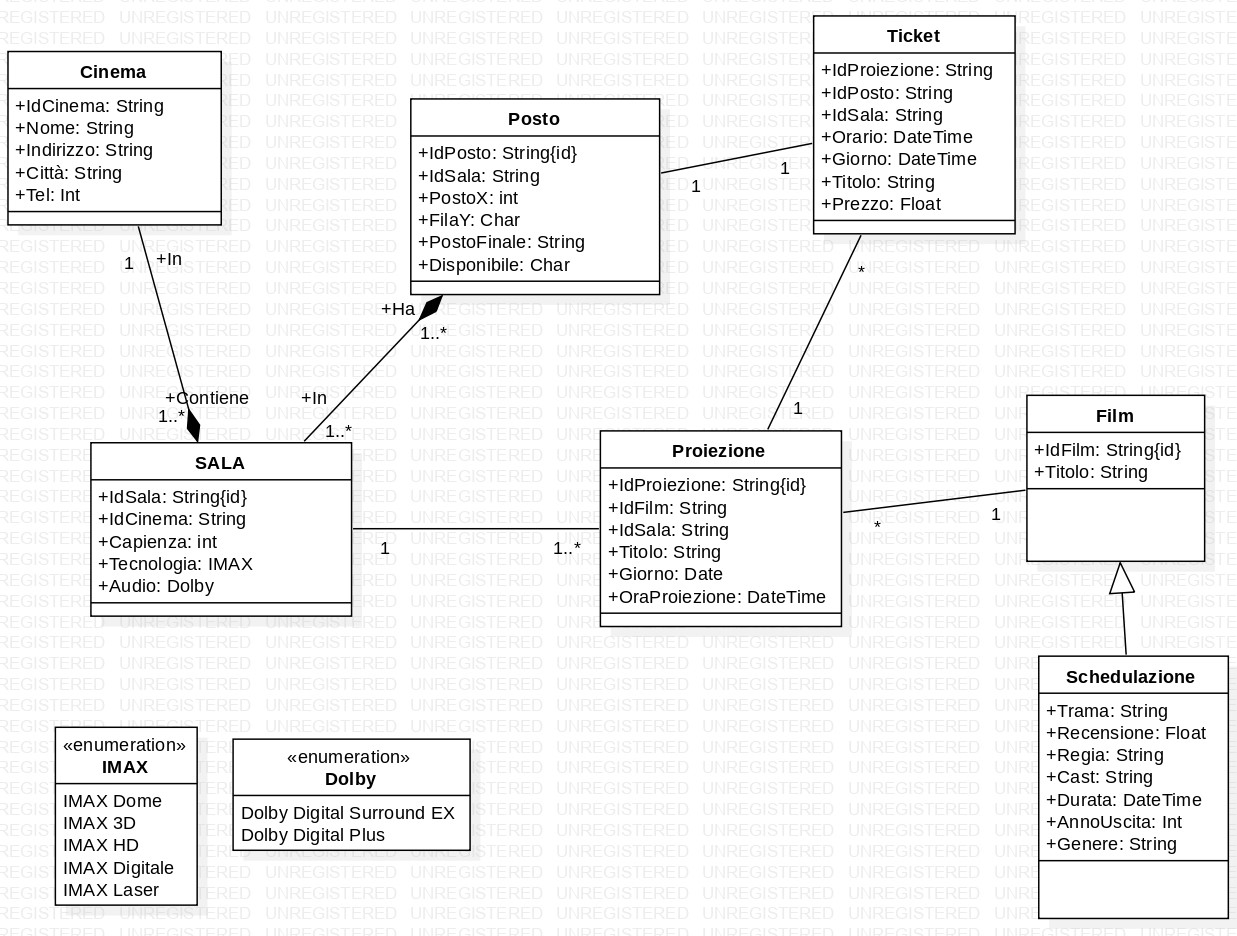
\includegraphics[width = 400pt, height = 550pt]{UML}
	\section{Dizionario dei dati}
	\subsection[short title]{Dizionario delle classi}
	\begin{center}

	\begin{tabular}{l p{3cm} p{10cm}}
		\hline
		Classe& Descrizione& Attributi\\
		\hline
		Cinema& Descrittore di ciascun cinema presente in italia& \textbf{IdCinema} \textit{String}: Identifica univocamente ogni cinema
		\newline \textbf{Nome} \textit{String}: Indica il nome del cinema
		\newline \textbf{Indirizzo} \textit{String}: Indica l'indirizzo del cinema
		\newline \textbf{Città} \textit{String}: Indica la città dove risiede il cinema
		\newline \textbf{Tel} \textit{Integer}: Indica il numero di telefono del cinema \\
		\hline
		Sala& Descrittore di ciascuna sala presente nel cinema &
		\textbf{IdSala} \textit{String}: Identifica univocamente ogni sala del cinema
		\newline \textbf{Capienza} \textit{Integer}: Indica il massimo dei posti per sala
		\newline \textbf{Tecnologia} \textit{IMAX}: \\
		\hline
	\end{tabular}
	\end{center}
		
\end{document}
